\section*{Exercise 3}
\label{sec:exercise-3}

\subsection*{(a)}
\label{sec:a-2}
The plot of the profiles are presented in figure
\ref{fig:ex3-profiles}.
\begin{figure}[h]
  \centering
  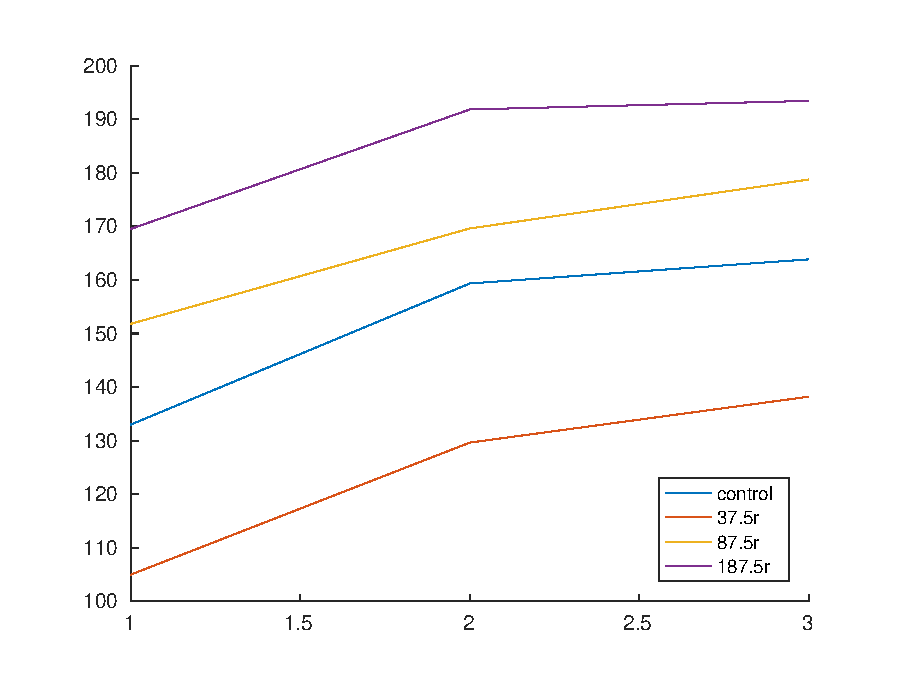
\includegraphics[width=8.5cm]{ex3-profiles}
  \caption{The profiles for the Psychomotor scores given different
    radiation treatment.}
  \label{fig:ex3-profiles}
\end{figure}

\subsection*{(b)}
\label{sec:b-2}

%Check the updated code, which should probably correct. 

To test if the profiles are parallel the test presented in Lecture
7 is used. First we introduce the matrices
\begin{align*}
  \b A &=
         \begin{pmatrix}
           \b 1_{n_{1}}  & \b 0_{n_{1}}& \b 0_{n_{1}}& \b 0_{n_{1}} \\
           \b 0_{n_{2}} &  \b 1_{n_{2}}  &\b 0_{n_{2}}& \b 0_{n_{2}} \\
           \b 0_{n_{3}}& \b 0_{n_{3}}&  \b 1_{n_{3}}  & \b 0_{n_{3}} \\
           \b 0_{n_{4}}& \b 0_{n_{4}}& \b 0_{n_{4}} &   \b 1_{n_{4}}   \\ 
         \end{pmatrix} \\
  \b V &= \b X^{T} (\b I_{n}   -  \b A(\b A^{T}\b A)^{-1}\b A^{T}) \b X, \\
  \b C &=
         \begin{pmatrix}
           1 & -1 & 0 \\
           1 &  0 & -1
         \end{pmatrix}, \\
  \b Y &=
         \begin{pmatrix}
           \b \mu_{1} - \mu_{4} &\b \mu_{2} - \mu_{4} &\b \mu_{3} - \mu_{4} 
         \end{pmatrix} \\
  \b C_{Y}^{-1} &= \diag (n_{1}, n_{2}, n_{3}) - \frac{1}{n}   (n_{1},
                  n_{2}, n_{3})^{T} (n_{1}, n_{2}, n_{3}), \\
  \b H &= \b Y\b C_{Y}^{-1}\b Y^{T}                  
\end{align*}
Then we construct the test statistic
\begin{equation*}
  Q = -
  \left(
    n - \frac{1}{2}(k + p + 1)
  \right)
  \left(
    \ln \abs{\b {CVC}^{T}} - \ln \abs{\b{CVC}^{T} + \b{CHC}^{T}}
  \right) ,
\end{equation*}
where we reject $H_{1}: $ \textit{the profiles are parallel} if $Q$ is larger
than 
\begin{equation*}
  c = \chi^{2}_{(p-1)(k-1)}(1 - \alpha), \quad \alpha = 0.05.
\end{equation*}
Since $Q =4.0443 $ and $c = 12.5916$, we cannot reject $H_{1}$, the
profiles are parallel


\subsection*{(c)}
\label{sec:c-2}

Since, the profiles are parallel, we can set up a test for checking if
the profiles are on the same level. The likelihood ratio is 
\begin{equation*}
  \lambda_{H_2 | H_1} = \frac{\abs{\b C\b V \b C^{T} + \b C \b H\b C^T}}{\abs{\b
      C\b V \b C^T}}\frac{\abs{\b V}}{\abs{\b V+\b H}},
\end{equation*}
from which $H_{2}|H_{1}$ is rejected if 
\begin{equation*}
  Q = \left(\frac{n-k - p +1}{k - 1}\right)\frac{1 - \lambda_{H_2 |H_1}}{\lambda_{H_2 | H_1}},
\end{equation*}
is larger then 
\begin{equation*}
  c = F_{k-1, n - k - p +1} (1 - \alpha), \quad \alpha = 0.05
\end{equation*}
We get
\begin{equation*}
 7.9361  = Q < c = 3.2145,
\end{equation*}
so $H_2 | H_1$ is rejected, the profiles are not on the same level.

\subsection*{(d)}
\label{sec:d-1}

Here, we use the test variables 
\begin{equation*}
  \lambda_{H_3 | H_1} = \frac{1}{1 + n \bar{\bf x}^T \b C^T (\b{CVC}^T +
    \b{CHC}^T)^{-1}}\b C\bar{\bf x},
\end{equation*}
and create the test variable
\begin{equation*}
  Q = \frac{n - p +1}{p - 1}\lambda_{H_3 |H_1}, 
\end{equation*}
which we compare to 
\begin{equation*}
  c = F_{p-1, n-p+1}(0.95).x
\end{equation*}
We get
\begin{equation*}
  7.9361 = Q > c = 3.2145.
\end{equation*}
Thus $H_3 | H_1$ is rejected, the profiles are not flat.
%%% Local Variables:
%%% mode: latex
%%% TeX-master: "examination"
%%% End:
